% !TEX encoding = UTF-8 Unicode
%!TEX TS-program = xelatex

\documentclass[12pt]{extarticle}
% extarticle is like article but can handle 8pt, 9pt, 10pt, 11pt, 12pt, 14pt, 17pt, and 20pt text

\def \ititle {Origins of Mind}
 
\def \isubtitle {Lecture 08}
 
\def \iauthor {Stephen A. Butterfill}
\def \iemail{s.butterfill@warwick.ac.uk}
\date{}

%for strikethrough
\usepackage[normalem]{ulem}

\usepackage{pdfpages}


\input{$HOME/Documents/submissions/preamble_steve_handout}

%logic symbol \leftmodels
\usepackage{MnSymbol}

%\bibpunct{}{}{,}{s}{}{,}  %use superscript TICS style bib
%remove hanging indent for TICS style bib
%TODO doesnt work
\setlength{\bibhang}{0em}
%\setlength{\bibsep}{0.5em}


%itemize bullet should be dash
\renewcommand{\labelitemi}{$-$}

\begin{document}

%\raggedcolumns

\begin{multicols*}{3}

\setlength\footnotesep{1em}


\bibliographystyle{newapa} %apalike

%\maketitle
%\tableofcontents




%--------------- 
%--- start paste
\def \ititle {Logic I}
 
\def \isubtitle {Lecture 2}
 
\begin{center}
 
{\Large
 
\textbf{\ititle}: \isubtitle
 
}
 
 
 
\iemail %
 
\end{center}
 
Readings refer to sections of the course textbook, \emph{Language, Proof and Logic}.
 
 
 
\section{Why Logic?}
 
‘Logic pervades the world: the limits of the world are also its limits.’
(Wittgenstein, Tractatus 5.61)
 
‘If a card has a vowel on one side, then it has an even number on the other side.’
(Waison \& Johnson-Laird 1972)
 
\begin{center}

\includegraphics[scale=0.3]{img/waison_fig.png}
\end{center}
 
 
\section{Recap: Validity, Counterexamples}
 
An argument is \emph{logically valid} just if there’s no possible situation in which the premises are true and the conclusion false
 
A \emph{counterexample} to an argument is a possible situation in which its premises are T and its conclusion F.
 
 
 
\section{Logical Validity and Truth Tables}
 
\emph{Reading:} §4.3
 
\begin{minipage}{\columnwidth}
 
Truth tables can be used to show that an argument is valid. To illustrate ...
 
\begin{center}
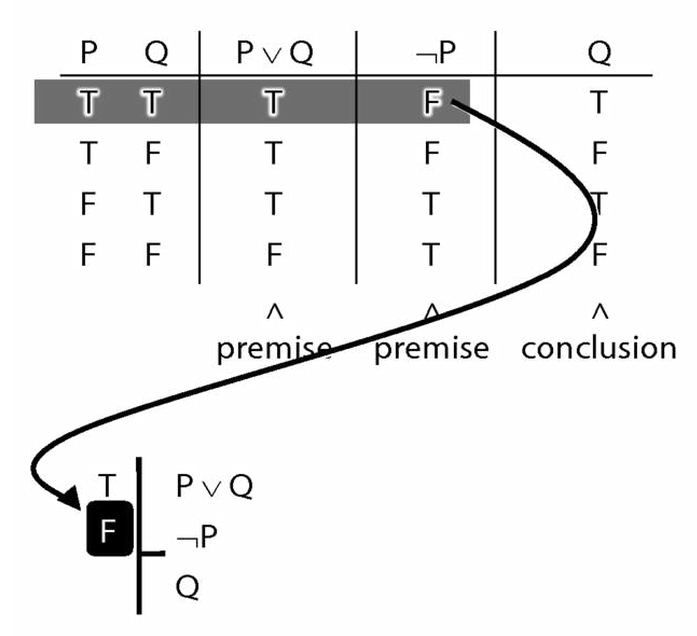
\includegraphics[scale=0.3]{img/unit_14_example.png}
\end{center}
\end{minipage}
 
\begin{minipage}{\columnwidth}
 
To establish that an argument is valid:
 
\begin{enumerate}
 
\item Create truth tables for each premise and the conclusion.
 
\item Check whether there is a row of the truth table where all premises are true and the conclusion is false.
 
\item If not, the argument is valid.
 
\end{enumerate}
 
\end{minipage}
 
 
 
\section{Complex Truth Tables}
 
\emph{Reading:} §3.3, §3.5
 
\begin{center}
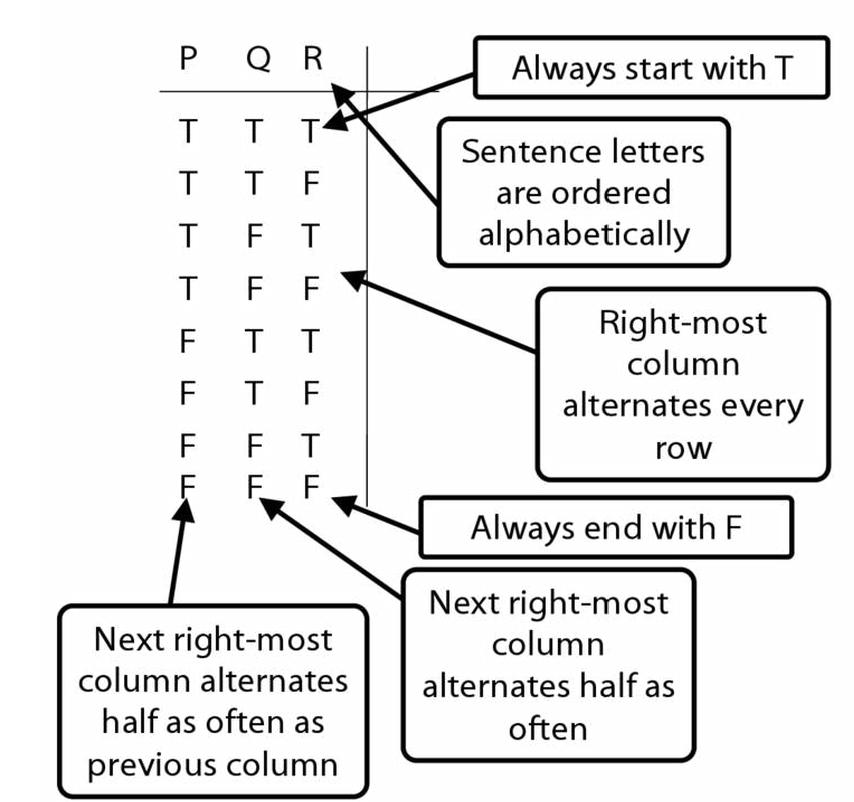
\includegraphics[scale=0.3]{img/how_to_write_truth_tables.png}
\end{center}
\begin{minipage}{\columnwidth}
 
Complex truth table example:
 
\begin{center}
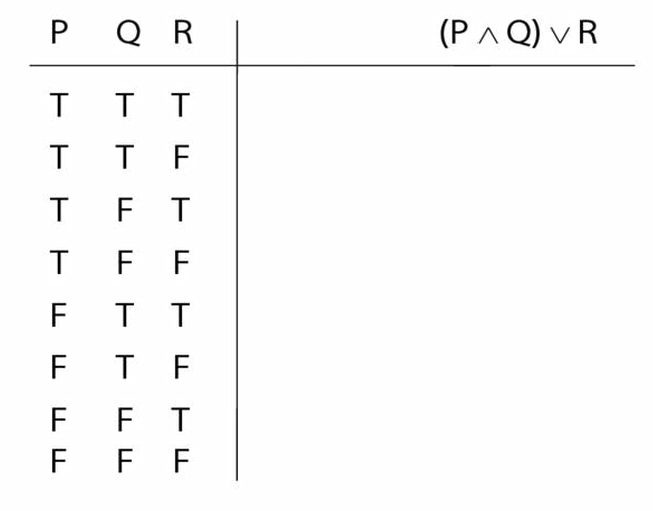
\includegraphics[scale=0.3]{img/tt_p_and_q_or_r.png}
\end{center}
\end{minipage}
 
 
 
\section{Tautologies and Contradictions}
 
\emph{Reading:} §4.1, §4.2
 
\begin{center}
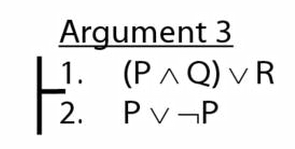
\includegraphics[scale=0.3]{img/unit_160_argument3.png}
\end{center}
\begin{center}
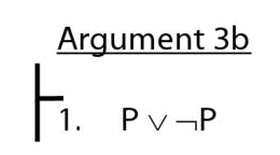
\includegraphics[scale=0.3]{img/unit_160_argument3b.png}
\end{center}
\begin{center}
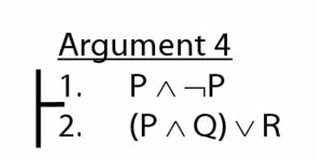
\includegraphics[scale=0.3]{img/unit_160_argument4.png}
\end{center}
P $\lor{}$ ¬P is a \emph{logical truth}
 
logical truth defined p. 568
 
P $\land{}$ ¬P is a \emph{contradiction}
 
contradiction defined p. 564
 
 
 
\section{Formal Proof: ∧Elim and ∧Intro}
 
\emph{Reading:} §5.1, §6.1
 
\begin{center}
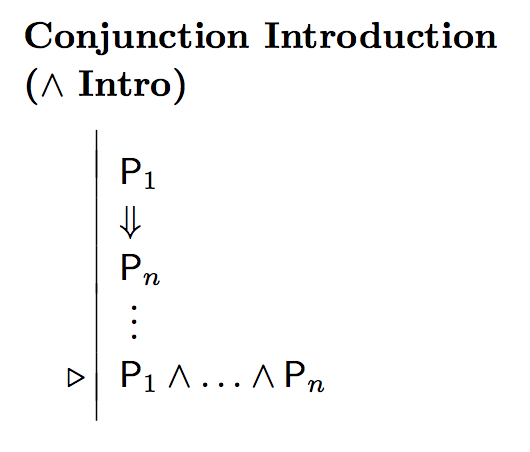
\includegraphics[scale=0.3]{img/rule_conjunction_intro.png}
\end{center}
\begin{center}
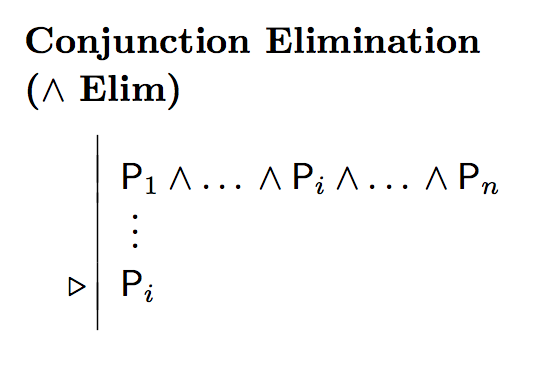
\includegraphics[scale=0.3]{img/rule_conjunction_elim.png}
\end{center}
\begin{center}
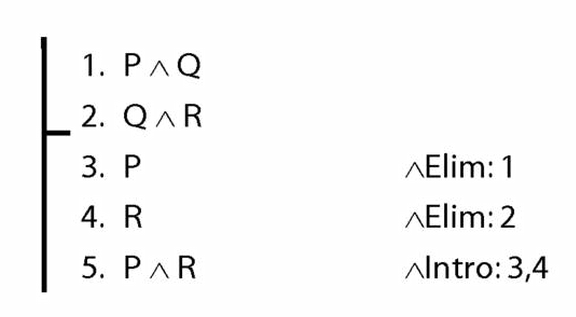
\includegraphics[scale=0.3]{img/proof_unit_21.png}
\end{center}
\vfill

%--- end paste
%--------------- 
 


\end{multicols*}

\end{document}